\subsection{\gls{crna} annotation}
In its minimal form, a \gls{crna} is defined by the chromosome it is located on
and the start and end position of the \gls{bsj}.
While this information is sufficient to uniquely identify a \gls{bsj}, it does
not provide any information about the gene or genes it is part of.
Furthermore, it does not give any information about the type of \gls{crna} it
is (types of \gls{crna} are described in \cref{sec:circrna_types}) and if it is
already has an entry in any \gls{crna} database.
While some tools like CircExplorer2 and DCC provide their own annotation, other
tools like find\_circ and segemehl do not.
To provide a consistent annotation for all \glspl{bsj}, \gls{nf-circrna} uses a
custom annotation process that will be described in the following sections.

\subsubsection{\gls{gtf}-based annotation}
\label{sec:gtf_annotation}
\gls{gtf} files are a common way to store genomic annotations like gene
locations and
transcript structures.
Such files are available for many reference genomes and can be used to identify
the genes and linear transcripts a \gls{crna} overlaps with.
This information can be used to infer the host gene(s) and the type of
\gls{crna}.

\begin{figure}[ht]
    \centering

    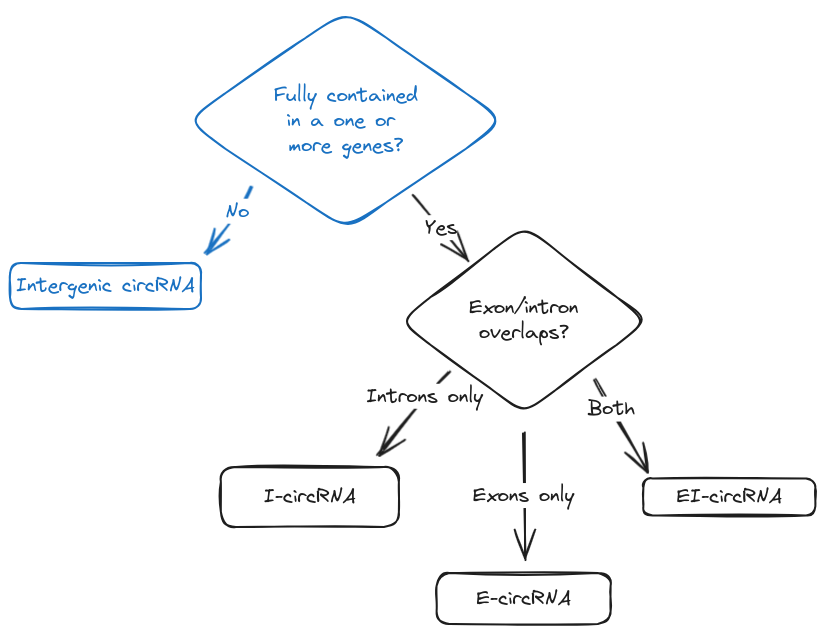
\includegraphics[width=\textwidth]{chapters/3_materials_and_methods/figures/annotation.png}
    \caption{Workflow of the \gls{gtf}-based \gls{crna} type annotation}
    \label{fig:gtf_annotation}
\end{figure}

The \gls{nf-circrna} pipeline identifies the type of \gls{crna} as shown in
\cref{fig:gtf_annotation}: \begin{enumerate} \item If the \gls{crna} does not
          overlap with any gene, it is labeled as \gls{ig-crna}.
    \item If the \gls{crna} is fully contained in any gene, the following
          classification is performed:
          \begin{itemize}
              \item If the \gls{crna} is fully contained in an exon, it is
                    labeled as \gls{e-crna}.
              \item If the \gls{crna} is fully contained in an intron, it
                    is
                    labeled as \gls{i-crna}.
              \item If the \gls{crna} spans both exonic and intronic
                    regions,
                    it is labeled as \gls{ei-crna}.
          \end{itemize}
\end{enumerate}

\subsubsection{Database-based annotation}
\label{sec:database_annotation}
In addition to \gls{gtf}-based annotation, \gls{nf-circrna} also provides
database-based annotation.
Databases like circBase and circAtlas store information about known
\glspl{crna}, often including functional
information\supercite{glazar_circbase_2014,wu_circatlas_2023}.
Most \gls{crna} databases provide their stored \glspl{crna} in form of a
\gls{bed} file, providing a fairly unified interface for tools to process their
stored information in an automated fashion.
\gls{nf-circrna} allows the user to provide an arbitrary number of such
\gls{bed}
files for database-based annotation.
The pipeline identifies a match between a detected \gls{crna} and a database
entry, if the bi-directional overlap is at least 90\%.
This means that at least 90\% of the detected \gls{crna} must overlap with the
database entry and vice versa.

In this study, the following databases were used for annotation:

\paragraph{circBase} circBase, established in 2014, was one of the first
databases dedicated to circRNAs.
It compiled data from nine large-scale studies, encompassing 92,375 circRNAs
from humans and key model organisms\supercite{glazar_circbase_2014}.
Although circBase was accessible at the beginning of this study, it has since
been taken offline.

\paragraph{circAtlas 3.0}
The third version of circAtlas was released in early 2024 and offers a more
extensive dataset with three million vertebrate circRNAs.
It covers ten species and 33 different tissues, providing valuable
cross-species conservation scores for researchers\supercite{wu_circatlas_2023}.
